% Schematische Draufsicht der Akku-Tischkreissäge, selbst gezeichnet (CC BY-SA 3.0).
% Keine maßstäbliche Abbildung: Die Nummern zeigen, welche Teile es gibt,
% nicht ihre exakte Lage an der Maschine.
% Nummern wie im Text: \teil{n}
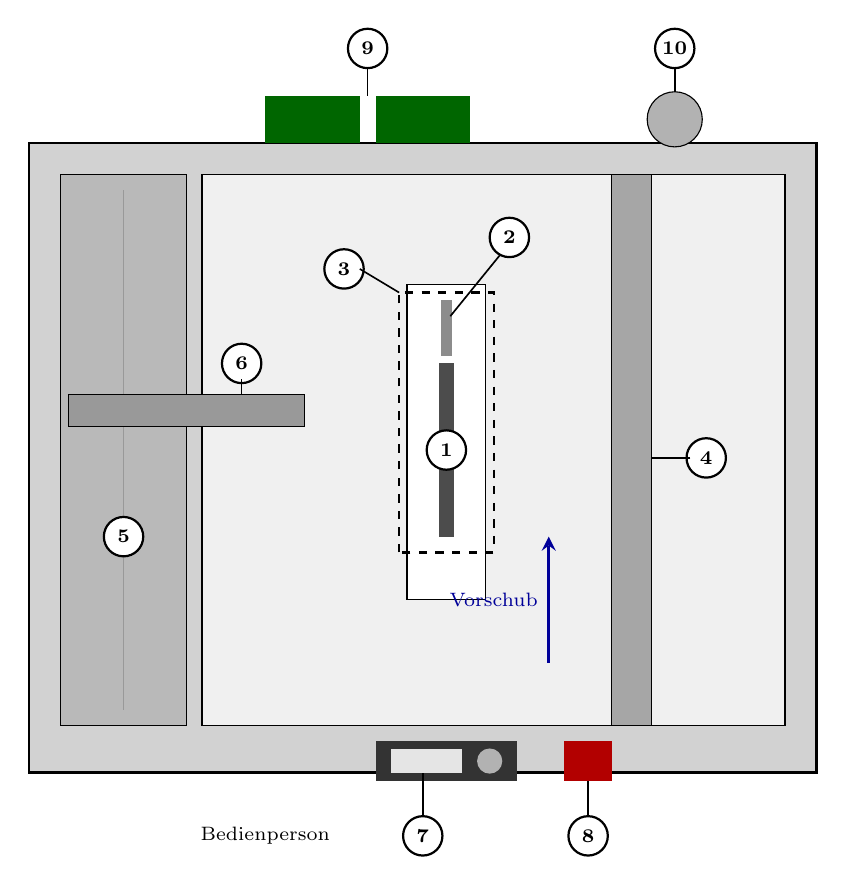
\begin{tikzpicture}[x=1mm, y=1mm, font=\sffamily\small,
		nr/.style={circle, draw=black, fill=white, line width=0.8pt, minimum size=5mm, inner sep=0pt, font=\scriptsize\bfseries},
		zeiger/.style={line width=0.6pt}]
	% Gehäuse (Systainer-Format)
	\fill[gray!35] (0,0) rectangle (100,80);
	\draw[line width=1pt] (0,0) rectangle (100,80);
	% Sägetisch
	\fill[gray!12] (22,6) rectangle (96,76);
	\draw[line width=0.6pt] (22,6) rectangle (96,76);
	% Schiebeschlitten links
	\fill[gray!55] (4,6) rectangle (20,76);
	\draw[line width=0.6pt] (4,6) rectangle (20,76);
	\draw[gray!80] (12,8) -- (12,74);
	% Winkelanschlag auf dem Schlitten
	\fill[gray!80] (5,44) rectangle (35,48);
	\draw (5,44) rectangle (35,48);
	% Tischeinlage mit Sägeblatt und Spaltkeil
	\fill[white] (48,22) rectangle (58,62);
	\draw (48,22) rectangle (58,62);
	\fill[black!70] (52,30) rectangle (54,52);
	\fill[gray!90] (52.3,53) rectangle (53.7,60);
	% Schutzhaube (durchsichtig) über dem Blatt
	\draw[dashed, line width=0.8pt] (47,28) rectangle (59,61);
	% Parallelanschlag rechts
	\fill[gray!70] (74,6) rectangle (79,76);
	\draw (74,6) rectangle (79,76);
	% Bedienfeld vorn: Display mit Drehrad, Schalter
	\fill[black!80] (44,-1) rectangle (62,4);
	\fill[gray!20] (46,0) rectangle (55,3);
	\fill[gray!60] (58.5,1.5) circle (1.6);
	\fill[red!70!black] (68,-1) rectangle (74,4);
	% Akkus und Absauganschluss hinten
	\fill[green!40!black] (30,80) rectangle (42,86);
	\fill[green!40!black] (44,80) rectangle (56,86);
	\fill[gray!60] (82,83) circle (3.5);
	\draw (82,83) circle (3.5);
	% Laufrichtung des Werkstücks
	\draw[-stealth, line width=1.2pt, blue!60!black] (66,14) -- (66,30) node[midway, left, font=\scriptsize] {Vorschub};
	% Nummern
	\node[nr] (n1) at (53,41) {1};
	\draw[zeiger] (60,66) -- (53.5,58); \node[nr] at (61,68) {2};
	\node[nr] at (40,64) {3}; \draw[zeiger] (42,64) -- (47,61);
	\node[nr] at (86,40) {4}; \draw[zeiger] (84,40) -- (79,40);
	\node[nr] at (12,30) {5};
	\node[nr] at (27,52) {6}; \draw[zeiger] (27,50) -- (27,48);
	\node[nr] at (50,-8) {7}; \draw[zeiger] (50,-5.5) -- (50,0);
	\node[nr] at (71,-8) {8}; \draw[zeiger] (71,-5.5) -- (71,-1);
	\node[nr] at (43,92) {9}; \draw[zeiger] (43,89.5) -- (43,86);
	\node[nr] at (82,92) {10}; \draw[zeiger] (82,89.5) -- (82,86.5);
	% Bedienposition
	\node[font=\scriptsize] at (30,-8) {Bedienperson};
\end{tikzpicture}
